\section{Mechanisms in the Oregon Health Insurance Experiment}
\label{sec:lottery}
In the United States, healthcare is generally not provided directly by the government.
Instead, consumers purchase health insurance to fund healthcare expenses, with the government providing insurance only for elderly individuals (Medicare) and for those with low-incomes (Medicaid).
In 2004, the state of Oregon ceased accepting new applications for Medicaid due to budgetary constraints, and did not reopen applications until 2008.
When the state resumed enrolment, 90,000 individuals applied, vastly exceeding the programme's capacity.
Oregon therefore allocated the opportunity to apply for Medicaid via a lottery system among those on the wait-list.
Winning this wait-list lottery significantly increased healthcare usage, plus self-reported health and happiness.

\begin{figure}[!htbp]
    \caption{Effects of the Wait-list Lottery in the Oregon Health Insurance Experiment.}
    \centering
    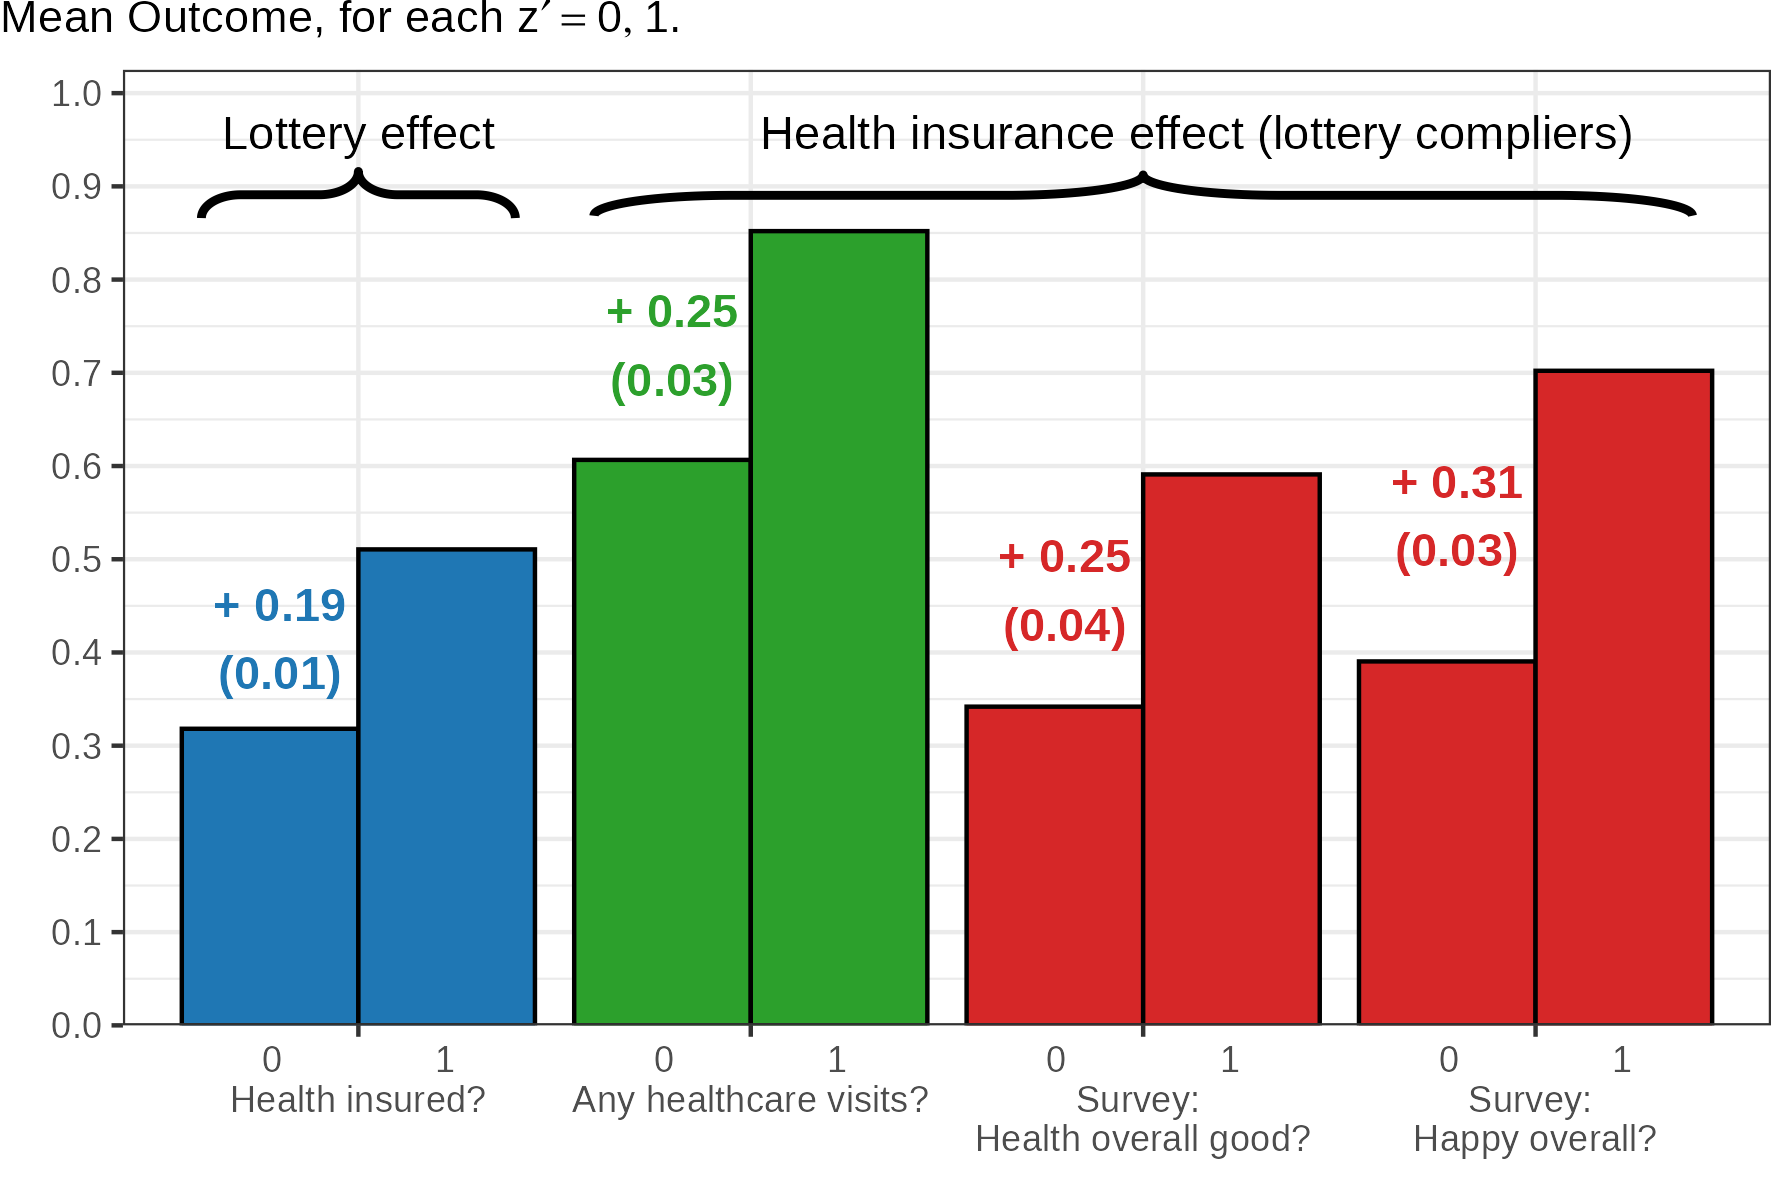
\includegraphics[width=0.85\textwidth]{sections/figures/insurance-effects.png}
    \label{fig:healthinsurance-effects}
    \justify
    \footnotesize    
    \textbf{Note:}
    This figure summarises the relevant results of the Oregon Health Insurance Experiment \citep{finkelstein2008oregon}.
    $\E{Y_i(z',.)}$ is the mean outcome, where $z' = 0$ refers to the case of losing the wait-list lottery (not given access to Medicaid), and $z' = 1$ winning.
    The numbers beside the bars are estimates of the mean difference; winning the Medicaid wait-list lottery increased average health insurance rate by 22 percentage points (pp), with standard errors of the difference reported in brackets.
\end{figure}

Winning the wait-list lottery increased the average health insurance coverage rate by 22 percentage points (pp), and self-reported visitation of any healthcare provider in the following 12 months by 5 pp.
In addition, wait-list lottery winners agreed 6 pp more with the question ``In general, would you say your health is excellent, very good, or good'' (hereafter, self-reported health),
and 5 pp for ``How would you say things are these days-would you say that you are very  or pretty happy'' (hereafter, self-reported happiness or well-being).
These figures are taken from the \input{../text/sections/tables/oregon-obs-count.txt} people from the Oregon wait-list lottery who responded to a survey sent by \cite{finkelstein2008oregon} one year later,\footnote{
    This number restricts to those who gave non-missing answers to all relevant questions.
}
calculated using the Oregon Health Insurance Experiment replication package \citep{icspr2014oregon}.
\autoref{fig:healthinsurance-effects} summarises these results.

These results show that winning the wait-list lottery led to large self-reported gains in both health and happiness.
The economics, medicine, and health policy literatures have primarily focused on the health benefits --- often interpreted as healthcare benefits from new access to government provided health insurance.\footnote{
    \cite{finkelstein2008oregon} use the wait-list lottery as an IV because health insurance is not randomly assigned; this paper focuses on the average effects of winning the wait-list lottery (which is randomly assigned).
}
However, the original authors also noted other benefits, including complete elimination of catastrophic out-of-pocket medical debt among those with new access to Medicaid.
% this was later followed up null results for the effect of health insurance on on clinically measured health outcomes \citep{baicker2013oregon}.
These are plausibly income effects that benefit recipients directly, not only through increased use of healthcare, but also by reducing stress and improving financial security.
These plausible direct effects have not been explored in the applied literature.

Accepted practice in applied economics is to investigate mechanisms behind causal effects with suggestive evidence.
This involves estimating the average causal effect of the wait-lottery on a proposed mediator (healthcare usage) and separately estimating its effect on the final outcomes (self-reported health and happiness).
When both estimates are positive, and the mediator precedes the outcome, it is taken as de facto evidence that the mediator transmits the treatment effect.
In the case of the Oregon Health Insurance Experiment, this amounts to concluding that increased healthcare usage mediates the positive effects of winning the lottery on health and happiness.
\autoref{fig:scm-health} illustrates this approach, which is also prevalent in other social science fields --- see \cite{blackwell2024assumption,green2010enough}.

\begin{figure}[!h]
    \centering
    \singlespacing
    \caption{Structural Causal Model for Suggestive Evidence of a Mechanism.}
    \label{fig:scm-health}
    \begin{tikzpicture}
        \node[state,thick,ForestGreen] (mediator) at (0,0) {$D_i$};
        \node[state,thick,blue] (treatment) [left=2.5cm of mediator] {$Z_i$};
        \node[state,thick,red] (outcome)   [right=2.5cm of mediator] {$Y_i$};
        % Label Z_i, D, Y_i
        \node[color=ForestGreen] [above=0.1cm of mediator] {Healthcare};
        \node[color=blue] [left=0.1cm of treatment] {Wait-list lottery};
        \node[color=red] [right=0.1cm of outcome] {Health \& Happiness};
        % Draw the causal arrows
        \path[->, thick] (treatment) edge (mediator);
        %\path[->, dashed,color=gray] (mediator) edge (outcome);
        \path[->, thick] (treatment) edge[bend right=30] (outcome);
        % Label the IV.
        %\node[state,thick,RoyalPurple] (treatmentIV) [above=0.75cm of treatment] {IV};
        %\node[color=RoyalPurple] [left=0.1cm of treatmentIV] {Wait-list lottery};
        %\path[->,thick,color=RoyalPurple] (treatmentIV) edge (treatment);
    \end{tikzpicture}
    \justify
    \footnotesize
    \textbf{Note}:
    This figure shows the structural causal model behind a suggestive analysis for effects of the Oregon Health Insurance Experiment, where arrows represent causal effects --- e.g., $Z_i \to D_i$ means $Z_i$ affects $D_i$ with no reverse causality.
\end{figure}

There are two main problems with this approach.
First, it provides no evidence for the effect of healthcare on health and well-being, so does not identify the causal mechanism.
Claims of identifying the mechanism (even suggestively) would require a hidden assumption that healthcare positively affects health outcomes.
While this assumption is not unreasonable, nowhere else in applied economics is a hidden assumption of a positive average causal effect taken at face value --- it must be motivated with quantitative evidence.
Second, this approach does not quantify the mechanism effects.
The proportion of effects operating through healthcare could only have a small effect on self-reported outcomes recorded only 12 months later, or possibly a very large effect --- it is a priori unclear.
In addition, the relevant mediating effect is not the average effect of healthcare usage, but the effect for Oregon residents who were induced to use more healthcare after winning the wait-list lottery. 
This local effect could differ substantially from a population average, and potentially mislead conclusions about the magnitude or generality of the mechanism.
In summary, this approach is not suggestive evidence of mechanisms, it is suggestive conjecture of mechanisms; it compels claims about mechanisms behind treatment effects which are not justified by causal evidence.

% Paragraph here to describe the percent of papers that do this.
% As well as the number of papers who just blatantly control for the mediator, too.

CM offers a compelling alternative framework.
Unlike suggestive evidence of mechanisms, CM explicitly defines the estimands of interest (the average direct and indirect effects) and lays out clear assumptions under which these quantities are identified.
Moreover, it delivers quantitative answers to the key question: how much of a treatment effect operates through a specific mediator mechanism?
CM is widely used in fields such as epidemiology, psychology, and medicine where researchers regularly decompose treatment effects into component pathways.
However, CM methods have not yet been rigorously examined from an economic perspective to assess their applicability in observational causal research, such as natural experiments.
